\chapter{Estimation of Active Sources}
\begin{itemize}
\item Here the simulated data is specified by $M=8,N=8,k=4$. But we still define $M=N=k$, as such we ask for 8 source, but there only 4. 
\item now the question is if we can identify k from the resulting plot.  
\item the mse is close to 0, indicating the the estimate is true, and from the plot we can see that the wrong estimates has very low amplitude, thus they will give a very low MSE when compare to a zero row.
\end{itemize}

\begin{figure}[H]
    \begin{minipage}[t]{.45\textwidth}
		\centering
		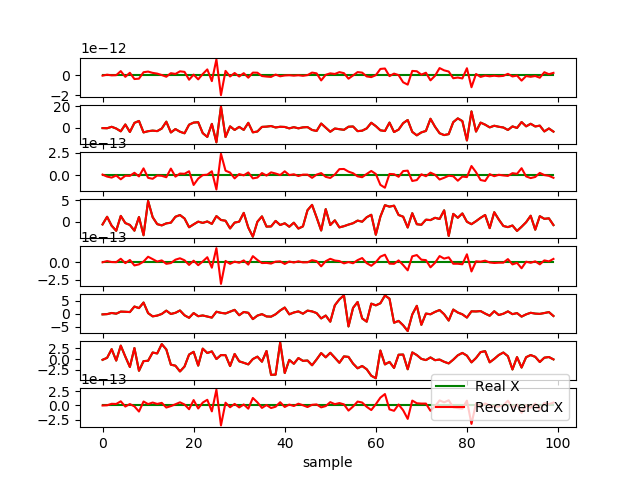
\includegraphics[scale=0.5]{figures/ch_7/M=N_testk=4.png}
	\caption{}
	\label{fig:M=N_k=4}
    \end{minipage} 
    \hfill
    \begin{minipage}[t]{.45\textwidth}
		\centering
		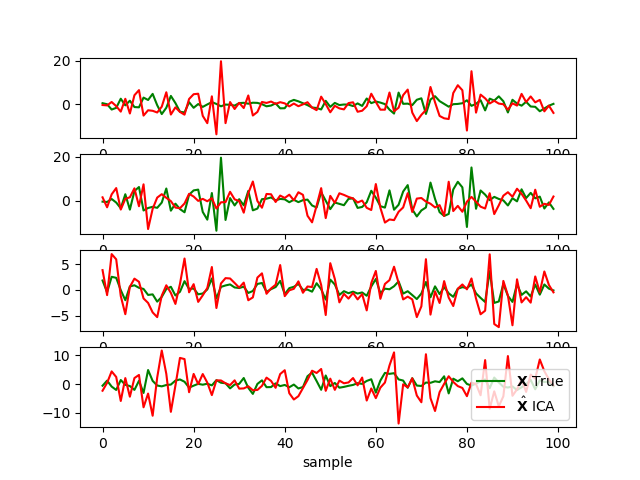
\includegraphics[scale=0.5]{figures/ICAapp/ICA_app4.png}
	\caption{}
	\label{fig:}
    \end{minipage}
\end{figure}
